<!DOCTYPE html>
<!-- Generated by pkgdown: do not edit by hand --><html lang="en"><head><meta http-equiv="Content-Type" content="text/html; charset=UTF-8"><meta charset="utf-8"><meta http-equiv="X-UA-Compatible" content="IE=edge"><meta name="viewport" content="width=device-width, initial-scale=1, shrink-to-fit=no"><meta name="description" content="Reproduce results from Yupana coding"><title>Yupana: coding workflow • inti</title><!-- favicons --><link rel="icon" type="image/png" sizes="16x16" href="../../favicon-16x16.png"><link rel="icon" type="image/png" sizes="32x32" href="../../favicon-32x32.png"><link rel="apple-touch-icon" type="image/png" sizes="180x180" href="../../apple-touch-icon.png"><link rel="apple-touch-icon" type="image/png" sizes="120x120" href="../../apple-touch-icon-120x120.png"><link rel="apple-touch-icon" type="image/png" sizes="76x76" href="../../apple-touch-icon-76x76.png"><link rel="apple-touch-icon" type="image/png" sizes="60x60" href="../../apple-touch-icon-60x60.png"><script src="../../deps/jquery-3.6.0/jquery-3.6.0.min.js"></script><meta name="viewport" content="width=device-width, initial-scale=1, shrink-to-fit=no"><link href="../../deps/bootstrap-5.3.1/bootstrap.min.css" rel="stylesheet"><script src="../../deps/bootstrap-5.3.1/bootstrap.bundle.min.js"></script><!-- Font Awesome icons --><link rel="stylesheet" href="https://cdnjs.cloudflare.com/ajax/libs/font-awesome/5.12.1/css/all.min.css" integrity="sha256-mmgLkCYLUQbXn0B1SRqzHar6dCnv9oZFPEC1g1cwlkk=" crossorigin="anonymous"><link rel="stylesheet" href="https://cdnjs.cloudflare.com/ajax/libs/font-awesome/5.12.1/css/v4-shims.min.css" integrity="sha256-wZjR52fzng1pJHwx4aV2AO3yyTOXrcDW7jBpJtTwVxw=" crossorigin="anonymous"><!-- bootstrap-toc --><script src="https://cdn.jsdelivr.net/gh/afeld/bootstrap-toc@v1.0.1/dist/bootstrap-toc.min.js" integrity="sha256-4veVQbu7//Lk5TSmc7YV48MxtMy98e26cf5MrgZYnwo=" crossorigin="anonymous"></script><!-- headroom.js --><script src="https://cdnjs.cloudflare.com/ajax/libs/headroom/0.11.0/headroom.min.js" integrity="sha256-AsUX4SJE1+yuDu5+mAVzJbuYNPHj/WroHuZ8Ir/CkE0=" crossorigin="anonymous"></script><script src="https://cdnjs.cloudflare.com/ajax/libs/headroom/0.11.0/jQuery.headroom.min.js" integrity="sha256-ZX/yNShbjqsohH1k95liqY9Gd8uOiE1S4vZc+9KQ1K4=" crossorigin="anonymous"></script><!-- clipboard.js --><script src="https://cdnjs.cloudflare.com/ajax/libs/clipboard.js/2.0.11/clipboard.min.js" integrity="sha512-7O5pXpc0oCRrxk8RUfDYFgn0nO1t+jLuIOQdOMRp4APB7uZ4vSjspzp5y6YDtDs4VzUSTbWzBFZ/LKJhnyFOKw==" crossorigin="anonymous" referrerpolicy="no-referrer"></script><!-- search --><script src="https://cdnjs.cloudflare.com/ajax/libs/fuse.js/6.4.6/fuse.js" integrity="sha512-zv6Ywkjyktsohkbp9bb45V6tEMoWhzFzXis+LrMehmJZZSys19Yxf1dopHx7WzIKxr5tK2dVcYmaCk2uqdjF4A==" crossorigin="anonymous"></script><script src="https://cdnjs.cloudflare.com/ajax/libs/autocomplete.js/0.38.0/autocomplete.jquery.min.js" integrity="sha512-GU9ayf+66Xx2TmpxqJpliWbT5PiGYxpaG8rfnBEk1LL8l1KGkRShhngwdXK1UgqhAzWpZHSiYPc09/NwDQIGyg==" crossorigin="anonymous"></script><script src="https://cdnjs.cloudflare.com/ajax/libs/mark.js/8.11.1/mark.min.js" integrity="sha512-5CYOlHXGh6QpOFA/TeTylKLWfB3ftPsde7AnmhuitiTX4K5SqCLBeKro6sPS8ilsz1Q4NRx3v8Ko2IBiszzdww==" crossorigin="anonymous"></script><!-- pkgdown --><script src="../../pkgdown.js"></script><meta property="og:title" content="Yupana: coding workflow"><meta property="og:description" content="Reproduce results from Yupana coding"><meta property="og:image" content="https://inkaverse.com/reference/figures/logo.png"><!-- mathjax --><script src="https://cdnjs.cloudflare.com/ajax/libs/mathjax/2.7.5/MathJax.js" integrity="sha256-nvJJv9wWKEm88qvoQl9ekL2J+k/RWIsaSScxxlsrv8k=" crossorigin="anonymous"></script><script src="https://cdnjs.cloudflare.com/ajax/libs/mathjax/2.7.5/config/TeX-AMS-MML_HTMLorMML.js" integrity="sha256-84DKXVJXs0/F8OTMzX4UR909+jtl4G7SPypPavF+GfA=" crossorigin="anonymous"></script><!--[if lt IE 9]>
<script src="https://oss.maxcdn.com/html5shiv/3.7.3/html5shiv.min.js"></script>
<script src="https://oss.maxcdn.com/respond/1.4.2/respond.min.js"></script>
<![endif]--><!-- Global site tag (gtag.js) - Google Analytics --><script async src="https://www.googletagmanager.com/gtag/js?id=G-804H2EJ8RN"></script><script>
  window.dataLayer = window.dataLayer || [];
  function gtag(){dataLayer.push(arguments);}
  gtag('js', new Date());

  gtag('config', 'G-804H2EJ8RN');
</script></head><body>
    <a href="#main" class="visually-hidden-focusable">Skip to contents</a>
    

    <nav class="navbar fixed-top navbar-light navbar-expand-lg bg-dark" data-bs-theme="light"><div class="container">
    
    <a class="navbar-brand me-2" href="../../index.html">inti</a>

    <small class="nav-text text-muted me-auto" data-bs-toggle="tooltip" data-bs-placement="bottom" title="">0.6.5</small>

    
    <button class="navbar-toggler" type="button" data-bs-toggle="collapse" data-bs-target="#navbar" aria-controls="navbar" aria-expanded="false" aria-label="Toggle navigation">
      <span class="navbar-toggler-icon"></span>
    </button>

    <div id="navbar" class="collapse navbar-collapse ms-3">
      <ul class="navbar-nav me-auto"><li class="nav-item">
  <a class="nav-link" href="../../index.html">
    <span class="fa fa-home fa-lg"></span>
     
  </a>
</li>
<li class="nav-item">
  <a class="nav-link" href="../../articles/apps.html">
    <span class="fa fa-gamepad fa-lg"></span>
     
    Apps
  </a>
</li>
<li class="active nav-item dropdown">
  <a href="#" class="nav-link dropdown-toggle" data-bs-toggle="dropdown" role="button" aria-expanded="false" aria-haspopup="true" id="dropdown--articles">
    <span class="fa fa-book fa-lg"></span>
     
    Articles
  </a>
  <div class="dropdown-menu" aria-labelledby="dropdown--articles">
    <a class="dropdown-item" href="../../articles/tarpuy.html">Tarpuy: field-book experimental plans</a>
    <a class="dropdown-item" href="../../articles/yupana.html">Yupana: experimental design analysis</a>
    <a class="dropdown-item" href="../../articles/extra/yupana-coding.html">Yupana: coding workflow</a>
    <a class="dropdown-item" href="../../articles/rticles.html">Rticles: scientific documents with R</a>
    <div class="dropdown-divider"></div>
    <a class="dropdown-item" href="../../articles/heritability.html">Broad-sense heritability in plant breeding</a>
  </div>
</li>
<li class="nav-item">
  <a class="nav-link" href="../../articles/policy.html">
    <span class="fa fa-shield-alt fa-lg"></span>
     
    Privacy Policy
  </a>
</li>
<li class="nav-item">
  <a class="nav-link" href="../../reference/index.html">
    <span class="fa fa-file-code fa-lg"></span>
     
    Functions
  </a>
</li>
<li class="nav-item">
  <a class="nav-link" href="../../news/index.html">
    <span class="fa fa-file-alt fa-lg"></span>
     
    News
  </a>
</li>
      </ul><form class="form-inline my-2 my-lg-0" role="search">
        <input type="search" class="form-control me-sm-2" aria-label="Toggle navigation" name="search-input" data-search-index="../../search.json" id="search-input" placeholder="Search for" autocomplete="off"></form>

      <ul class="navbar-nav"><li class="nav-item">
  <a class="external-link nav-link" href="https://github.com/flavjack/inti/">
    <span class="fab fa fab fa-github fa-lg"></span>
     
  </a>
</li>
<li class="nav-item">
  <a class="external-link nav-link" href="https://github.com/sponsors/Flavjack">
    <span class="fas fa fas fa-heart fa-lg"></span>
     
  </a>
</li>
      </ul></div>

    
  </div>
</nav><div class="container template-article">


<div class="row">
  <main id="main" class="col-md-9"><div class="page-header">
      <img src="../../logo.png" class="logo" alt=""><h1>Yupana: coding workflow</h1>
                        <h4 data-toc-skip class="author">Flavio Lozano-Isla</h4>
            
      
      <small class="dont-index">Source: <a href="https://github.com/flavjack/inti/blob/HEAD/vignettes/extra/yupana-coding.Rmd" class="external-link"><code>vignettes/extra/yupana-coding.Rmd</code></a></small>
      <div class="d-none name"><code>yupana-coding.Rmd</code></div>
    </div>

    
    
\section{Packages}\label{packages}

\begin{Shaded}
\begin{Highlighting}[]
\FunctionTok{library}\NormalTok{(inti)}
\FunctionTok{library}\NormalTok{(gsheet)}
\FunctionTok{library}\NormalTok{(FactoMineR)}
\FunctionTok{library}\NormalTok{(cowplot)}
\FunctionTok{library}\NormalTok{(png)}
\end{Highlighting}
\end{Shaded}

\section{Import data}\label{import-data}

\begin{Shaded}
\begin{Highlighting}[]
\NormalTok{url }\OtherTok{\textless{}{-}} \FunctionTok{paste0}\NormalTok{(}\StringTok{"https://docs.google.com/spreadsheets/d/"}
\NormalTok{              , }\StringTok{"15r7ZwcZZHbEgltlF6gSFvCTFA{-}CFzVBWwg3mFlRyKPs/edit\#gid=172957346"}\NormalTok{) }

\CommentTok{\# browseURL(url)}

\NormalTok{fb }\OtherTok{\textless{}{-}}\NormalTok{ url }\SpecialCharTok{\%\textgreater{}\%} 
  \FunctionTok{gsheet2tbl}\NormalTok{() }\SpecialCharTok{\%\textgreater{}\%} 
  \FunctionTok{rename\_with}\NormalTok{(tolower) }\SpecialCharTok{\%\textgreater{}\%} 
  \FunctionTok{mutate}\NormalTok{(}\FunctionTok{across}\NormalTok{(}\FunctionTok{c}\NormalTok{(riego, geno, bloque), }\SpecialCharTok{\textasciitilde{}} \FunctionTok{as.factor}\NormalTok{(.))) }\SpecialCharTok{\%\textgreater{}\%} 
  \FunctionTok{mutate}\NormalTok{(}\FunctionTok{across}\NormalTok{(}\FunctionTok{where}\NormalTok{(is.factor), }\SpecialCharTok{\textasciitilde{}} \FunctionTok{gsub}\NormalTok{(}\StringTok{"[[:space:]]"}\NormalTok{, }\StringTok{""}\NormalTok{, .)) ) }\SpecialCharTok{\%\textgreater{}\%} 
  \FunctionTok{as.data.frame}\NormalTok{()}
\CommentTok{\# str(fb)}
\end{Highlighting}
\end{Shaded}

\section{Plot raw data}\label{plot-raw-data}

\subsection{Box plot}\label{box-plot}

\begin{Shaded}
\begin{Highlighting}[]
\NormalTok{wue }\OtherTok{\textless{}{-}}\NormalTok{ fb }\SpecialCharTok{\%\textgreater{}\%} 
  \FunctionTok{plot\_raw}\NormalTok{(}\AttributeTok{type =} \StringTok{"boxplot"}
\NormalTok{           , }\AttributeTok{x =} \StringTok{"geno"}
\NormalTok{           , }\AttributeTok{y =} \StringTok{"wue"}
\NormalTok{           , }\AttributeTok{group =} \StringTok{"riego"}
\NormalTok{           , }\AttributeTok{xlab =} \StringTok{"Genotipos"}
\NormalTok{           , }\AttributeTok{ylab =} \StringTok{"Water use efficiency (g/l)"}
\NormalTok{           , }\AttributeTok{ylimits =} \FunctionTok{c}\NormalTok{(}\DecValTok{5}\NormalTok{, }\DecValTok{30}\NormalTok{, }\DecValTok{5}\NormalTok{)}
\NormalTok{           , }\AttributeTok{glab =} \StringTok{"Tratamientos"}
\NormalTok{           )}
\end{Highlighting}
\end{Shaded}

\subsection{Scatter plot}\label{scatter-plot}

\begin{Shaded}
\begin{Highlighting}[]
\NormalTok{hi }\OtherTok{\textless{}{-}}\NormalTok{ fb }\SpecialCharTok{\%\textgreater{}\%} 
  \FunctionTok{plot\_raw}\NormalTok{(}\AttributeTok{type =} \StringTok{"scatterplot"}
\NormalTok{           , }\AttributeTok{x =} \StringTok{"hi"}
\NormalTok{           , }\AttributeTok{y =} \StringTok{"twue"}
\NormalTok{           , }\AttributeTok{group =} \StringTok{"riego"}
\NormalTok{           , }\AttributeTok{xlab =} \StringTok{"Harvest Index"}
\NormalTok{           , }\AttributeTok{ylab =} \StringTok{"Tuber water use efficiency (g/l)"}
\NormalTok{           , }\AttributeTok{glab =} \StringTok{"Tratamientos"}
\NormalTok{           )}
\end{Highlighting}
\end{Shaded}

\subsection{Plot in grids}\label{plot-in-grids}

\begin{Shaded}
\begin{Highlighting}[]
\NormalTok{grid }\OtherTok{\textless{}{-}} \FunctionTok{plot\_grid}\NormalTok{(wue, hi}
\NormalTok{                  , }\AttributeTok{nrow =} \DecValTok{2}
\NormalTok{                  , }\AttributeTok{labels =} \StringTok{"AUTO"}\NormalTok{)}

\FunctionTok{save\_plot}\NormalTok{(}\StringTok{"files/fig{-}01.png"}
\NormalTok{        , }\AttributeTok{plot =}\NormalTok{ grid}
\NormalTok{        , }\AttributeTok{dpi=} \DecValTok{300}
\NormalTok{        , }\AttributeTok{base\_width =} \DecValTok{10}
\NormalTok{        , }\AttributeTok{base\_height =} \DecValTok{10}
\NormalTok{        , }\AttributeTok{scale =} \FloatTok{1.4}
\NormalTok{        , }\AttributeTok{units =} \StringTok{"cm"}
\NormalTok{        )}

\NormalTok{knitr}\SpecialCharTok{::}\FunctionTok{include\_graphics}\NormalTok{(}\StringTok{"files/fig{-}01.png"}\NormalTok{)}
\end{Highlighting}
\end{Shaded}

\begin{figure}

{\centering 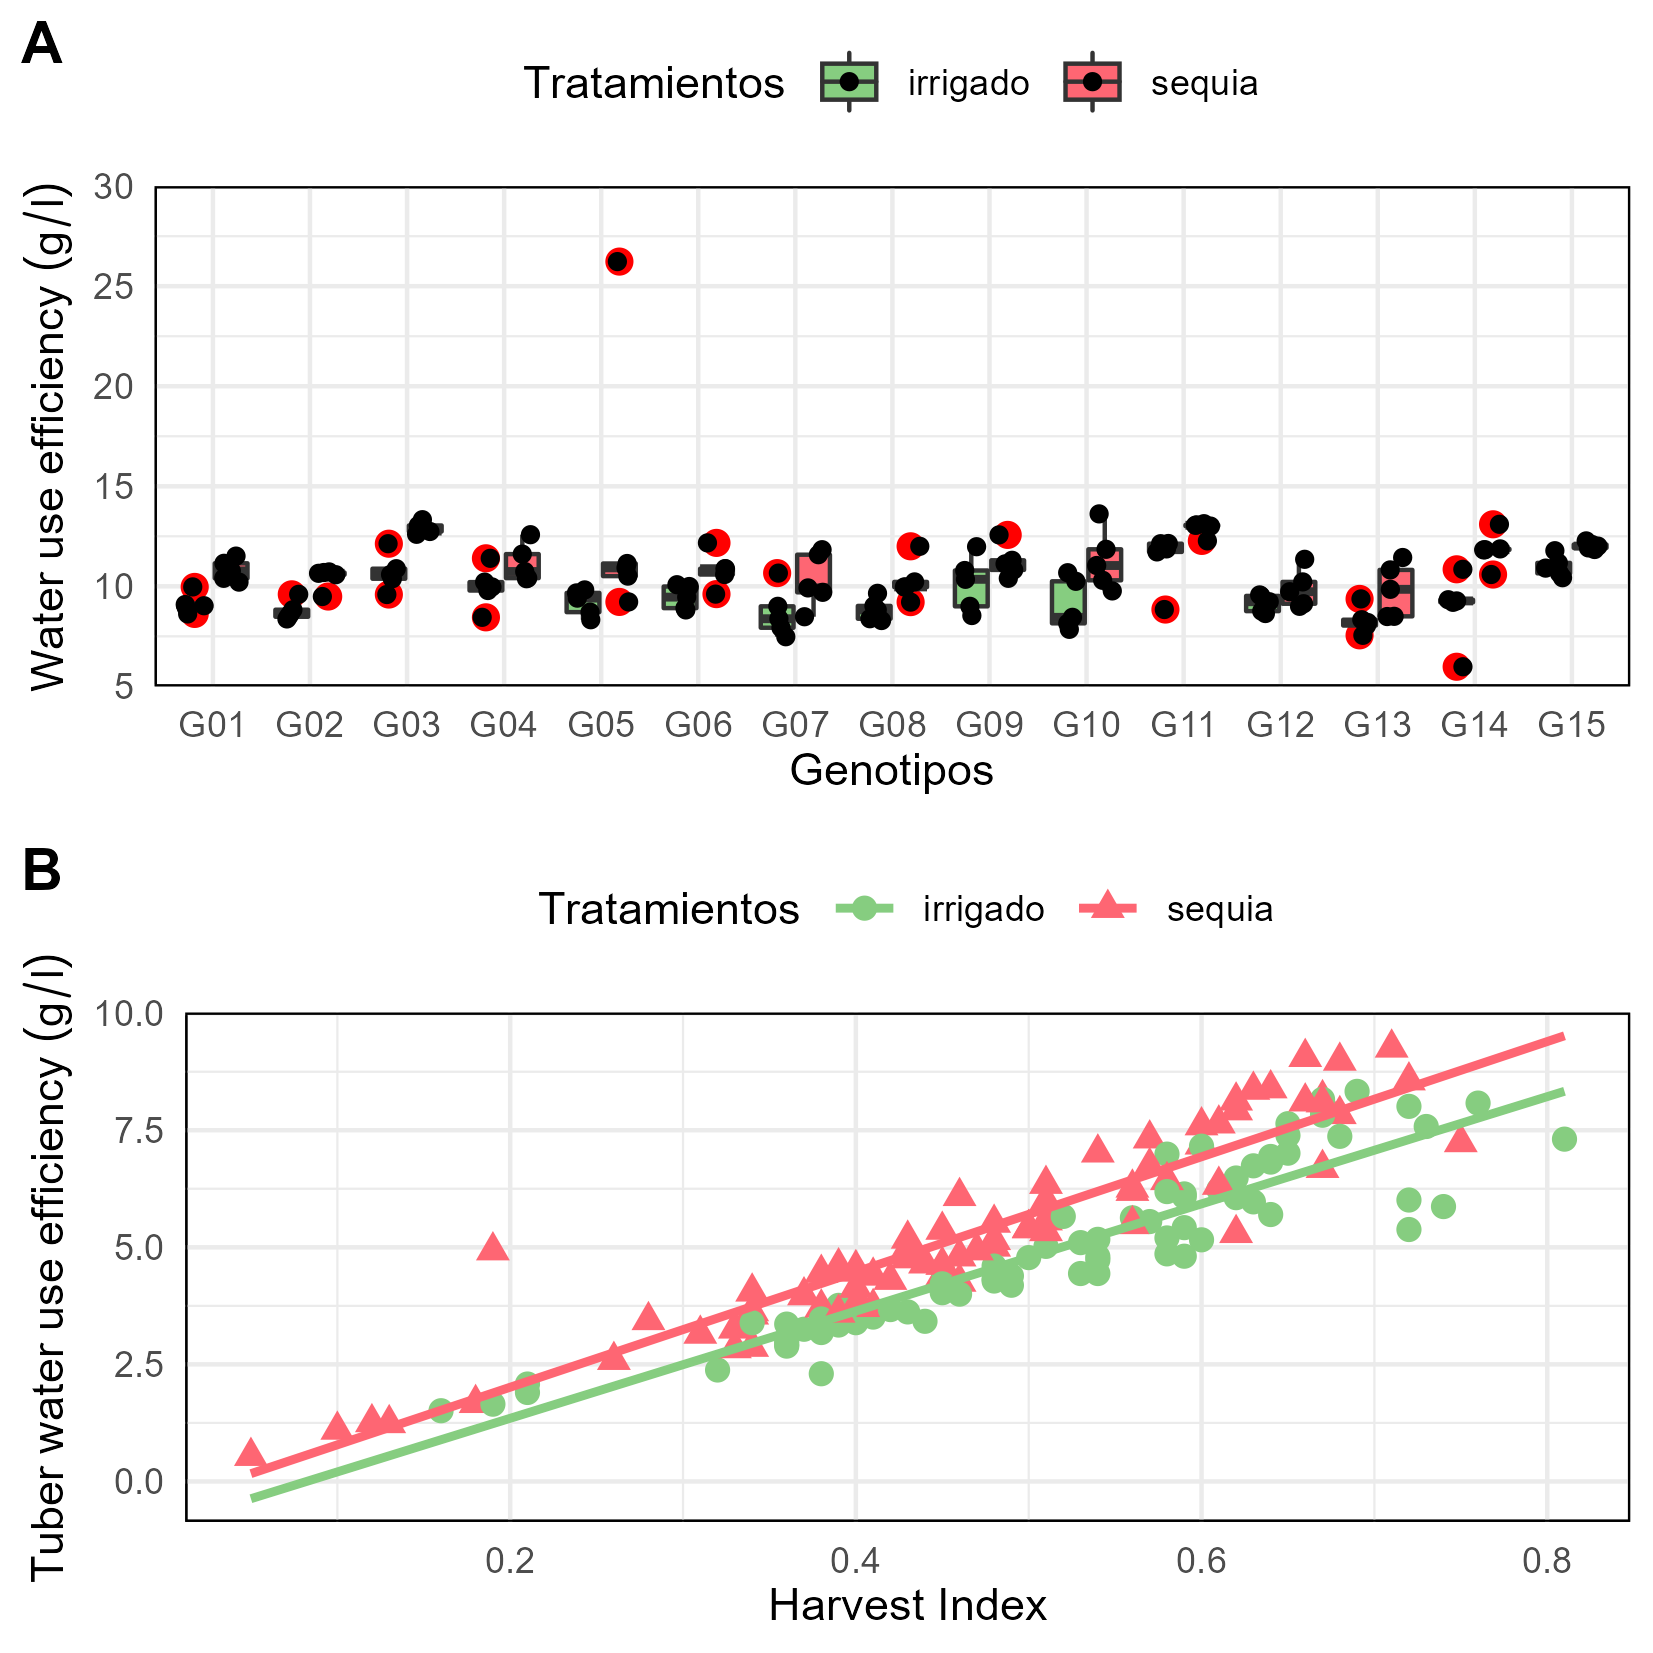
\includegraphics[width=0.98\linewidth]{files/fig-01} 

}

\caption{Water use effiency in 15 potato genotypes A) Box plot B) Scatter plot.}(\#fig:unnamed-chunk-5)
\end{figure}

\section{Plot summary data}\label{plot-summary-data}

\subsection{Leaf area}\label{leaf-area}

\begin{Shaded}
\begin{Highlighting}[]

\CommentTok{\#\textgreater{} Plot summary data}

\NormalTok{model }\OtherTok{\textless{}{-}}\NormalTok{ fb }\SpecialCharTok{\%\textgreater{}\%} 
  \FunctionTok{yupana\_analysis}\NormalTok{(}\AttributeTok{response =} \StringTok{"lfa"}
\NormalTok{                  , }\AttributeTok{model\_factors =} \StringTok{"geno*riego"}
\NormalTok{                  , }\AttributeTok{comparison =} \FunctionTok{c}\NormalTok{(}\StringTok{"geno"}\NormalTok{, }\StringTok{"riego"}\NormalTok{)}
\NormalTok{                  )}

\NormalTok{lfa }\OtherTok{\textless{}{-}}\NormalTok{ model}\SpecialCharTok{$}\NormalTok{meancomp }\SpecialCharTok{\%\textgreater{}\%} 
  \FunctionTok{plot\_smr}\NormalTok{(}\AttributeTok{type =} \StringTok{"bar"}
\NormalTok{           , }\AttributeTok{x =} \StringTok{"geno"}
\NormalTok{           , }\AttributeTok{y =} \StringTok{"lfa"}
\NormalTok{           , }\AttributeTok{group =} \StringTok{"riego"}
\NormalTok{           , }\AttributeTok{ylimits =} \FunctionTok{c}\NormalTok{(}\DecValTok{0}\NormalTok{, }\DecValTok{12000}\NormalTok{, }\DecValTok{2000}\NormalTok{)}
\NormalTok{           , }\AttributeTok{sig =} \StringTok{"sig"}
\NormalTok{           , }\AttributeTok{error =} \StringTok{"ste"}
\NormalTok{           , }\AttributeTok{xlab =} \StringTok{"Genotipos"}
\NormalTok{           , }\AttributeTok{ylab =} \StringTok{"Area foliar (cm\^{}2)"}
\NormalTok{           , }\AttributeTok{color =}\NormalTok{ F}
\NormalTok{           )}

\NormalTok{model}\SpecialCharTok{$}\NormalTok{anova }\SpecialCharTok{\%\textgreater{}\%} \FunctionTok{anova}\NormalTok{()}
\DocumentationTok{\#\# Analysis of Variance Table}
\DocumentationTok{\#\# }
\DocumentationTok{\#\# Response: lfa}
\DocumentationTok{\#\#             Df    Sum Sq   Mean Sq  F value                Pr(\textgreater{}F)    }
\DocumentationTok{\#\# geno        14 261742780  18695913   33.371 \textless{} 0.00000000000000022 ***}
\DocumentationTok{\#\# riego        1 788562704 788562704 1407.541 \textless{} 0.00000000000000022 ***}
\DocumentationTok{\#\# geno:riego  14 108153220   7725230   13.789 \textless{} 0.00000000000000022 ***}
\DocumentationTok{\#\# Residuals  120  67228987    560242                                   }
\DocumentationTok{\#\# {-}{-}{-}}
\DocumentationTok{\#\# Signif. codes:  0 \textquotesingle{}***\textquotesingle{} 0.001 \textquotesingle{}**\textquotesingle{} 0.01 \textquotesingle{}*\textquotesingle{} 0.05 \textquotesingle{}.\textquotesingle{} 0.1 \textquotesingle{} \textquotesingle{} 1}
\end{Highlighting}
\end{Shaded}

\begin{Shaded}
\begin{Highlighting}[]

\NormalTok{model}\SpecialCharTok{$}\NormalTok{meancomp }\SpecialCharTok{\%\textgreater{}\%} \FunctionTok{web\_table}\NormalTok{()}
\end{Highlighting}
\end{Shaded}

\subsection{Tuber water use efficiency}\label{tuber-water-use-efficiency}

\begin{Shaded}
\begin{Highlighting}[]
\NormalTok{model }\OtherTok{\textless{}{-}}\NormalTok{ fb }\SpecialCharTok{\%\textgreater{}\%} 
  \FunctionTok{yupana\_analysis}\NormalTok{(}\AttributeTok{response =} \StringTok{"twue"}
\NormalTok{                  , }\AttributeTok{model\_factors =} \StringTok{"block + geno*riego"}
\NormalTok{                  , }\AttributeTok{comparison =} \FunctionTok{c}\NormalTok{(}\StringTok{"geno"}\NormalTok{, }\StringTok{"riego"}\NormalTok{)}
\NormalTok{                  )}

\NormalTok{twue }\OtherTok{\textless{}{-}}\NormalTok{ model}\SpecialCharTok{$}\NormalTok{meancomp }\SpecialCharTok{\%\textgreater{}\%} 
  \FunctionTok{plot\_smr}\NormalTok{(}\AttributeTok{type =} \StringTok{"line"}
\NormalTok{           , }\AttributeTok{x =} \StringTok{"geno"}
\NormalTok{           , }\AttributeTok{y =} \StringTok{"twue"}
\NormalTok{           , }\AttributeTok{group =} \StringTok{"riego"}
\NormalTok{           , }\AttributeTok{ylimits =} \FunctionTok{c}\NormalTok{(}\DecValTok{0}\NormalTok{, }\DecValTok{10}\NormalTok{, }\DecValTok{2}\NormalTok{)}
\NormalTok{           , }\AttributeTok{error =} \StringTok{"ste"}
\NormalTok{           , }\AttributeTok{color =} \FunctionTok{c}\NormalTok{(}\StringTok{"blue"}\NormalTok{, }\StringTok{"red"}\NormalTok{)}
\NormalTok{           , }
\NormalTok{           ) }\SpecialCharTok{+}
  \FunctionTok{labs}\NormalTok{(}\AttributeTok{x =} \StringTok{"Genotipos"}
\NormalTok{       , }\AttributeTok{y =} \StringTok{"Tuber water use effiency (g/l)"}
\NormalTok{       )}

\NormalTok{model}\SpecialCharTok{$}\NormalTok{anova }\SpecialCharTok{\%\textgreater{}\%} \FunctionTok{anova}\NormalTok{()}
\DocumentationTok{\#\# Analysis of Variance Table}
\DocumentationTok{\#\# }
\DocumentationTok{\#\# Response: twue}
\DocumentationTok{\#\#             Df Sum Sq Mean Sq F value                Pr(\textgreater{}F)    }
\DocumentationTok{\#\# block        1  20.78 20.7770 31.0214          0.0000001609 ***}
\DocumentationTok{\#\# geno        14 413.06 29.5046 44.0523 \textless{} 0.00000000000000022 ***}
\DocumentationTok{\#\# riego        1   2.04  2.0370  3.0414               0.08375 .  }
\DocumentationTok{\#\# geno:riego  14  16.07  1.1479  1.7140               0.06138 .  }
\DocumentationTok{\#\# Residuals  119  79.70  0.6698                                  }
\DocumentationTok{\#\# {-}{-}{-}}
\DocumentationTok{\#\# Signif. codes:  0 \textquotesingle{}***\textquotesingle{} 0.001 \textquotesingle{}**\textquotesingle{} 0.01 \textquotesingle{}*\textquotesingle{} 0.05 \textquotesingle{}.\textquotesingle{} 0.1 \textquotesingle{} \textquotesingle{} 1}
\end{Highlighting}
\end{Shaded}

\begin{Shaded}
\begin{Highlighting}[]

\NormalTok{model}\SpecialCharTok{$}\NormalTok{meancomp }\SpecialCharTok{\%\textgreater{}\%} \FunctionTok{web\_table}\NormalTok{()}
\end{Highlighting}
\end{Shaded}

\subsection{Plot in grids}\label{plot-in-grids-1}

\begin{Shaded}
\begin{Highlighting}[]
\NormalTok{grid }\OtherTok{\textless{}{-}} \FunctionTok{plot\_grid}\NormalTok{(lfa, twue}
\NormalTok{                  , }\AttributeTok{nrow =} \DecValTok{2}
\NormalTok{                  , }\AttributeTok{labels =} \StringTok{"AUTO"}\NormalTok{)}

\FunctionTok{ggsave2}\NormalTok{(}\StringTok{"files/fig{-}02.png"}
\NormalTok{        , }\AttributeTok{plot =}\NormalTok{ grid}
\NormalTok{        , }\AttributeTok{dpi=} \DecValTok{300}
\NormalTok{        , }\AttributeTok{width =} \DecValTok{10}
\NormalTok{        , }\AttributeTok{height =} \DecValTok{10}
\NormalTok{        , }\AttributeTok{scale =} \FloatTok{1.5}
\NormalTok{        , }\AttributeTok{units =} \StringTok{"cm"}\NormalTok{)}

\NormalTok{knitr}\SpecialCharTok{::}\FunctionTok{include\_graphics}\NormalTok{(}\StringTok{"files/fig{-}02.png"}\NormalTok{)}
\end{Highlighting}
\end{Shaded}

\begin{figure}

{\centering 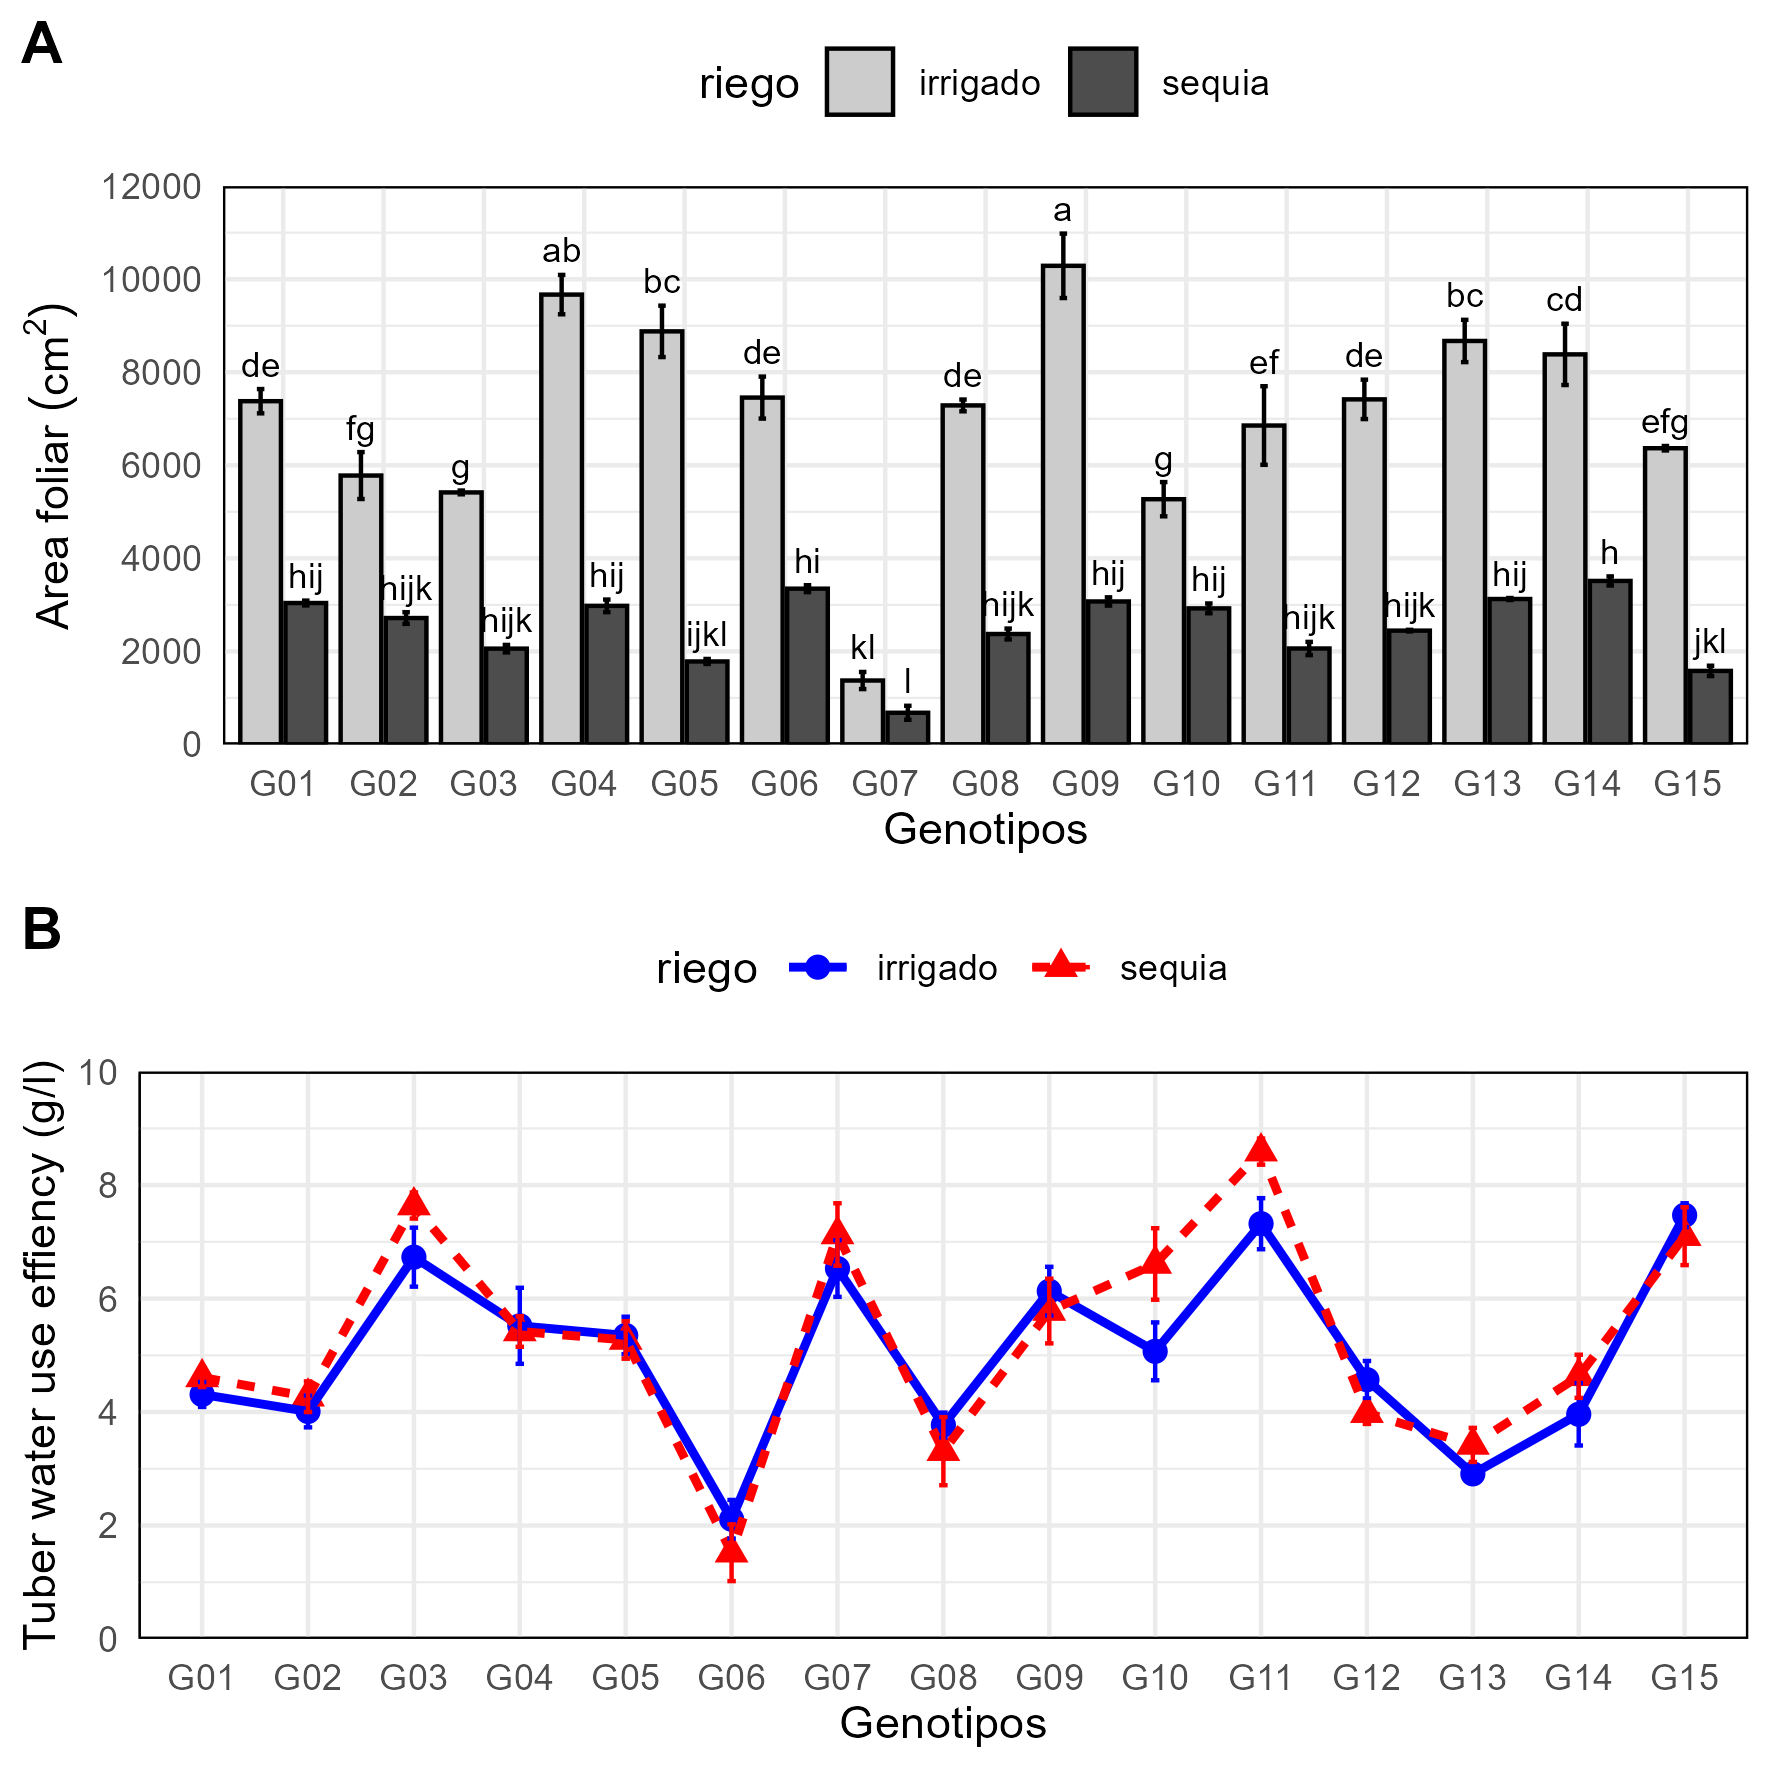
\includegraphics[width=0.98\linewidth]{files/fig-02} 

}

\caption{Water use effiency in 15 potato genotypes A) Bar plot B) Line plot.}(\#fig:gridplot)
\end{figure}

\section{Multivariate analysis}\label{multivariate-analysis}

\begin{Shaded}
\begin{Highlighting}[]
\CommentTok{\#\textgreater{} Principal component Analysis}

\NormalTok{mv }\OtherTok{\textless{}{-}}\NormalTok{ fb }\SpecialCharTok{\%\textgreater{}\%} 
  \FunctionTok{yupana\_mvr}\NormalTok{(}\AttributeTok{last\_factor =} \StringTok{"bloque"}
\NormalTok{             , }\AttributeTok{summary\_by =} \FunctionTok{c}\NormalTok{(}\StringTok{"geno"}\NormalTok{, }\StringTok{"riego"}\NormalTok{)}
\NormalTok{             , }\AttributeTok{groups =} \StringTok{"riego"}
\NormalTok{             )}
  
\CommentTok{\# sink("files/pca.txt")}
\CommentTok{\# \# Results}
\CommentTok{\# summary(pca, nbelements = Inf, nb.dec = 2)}
\CommentTok{\# \# Correlation de dimensions}
\CommentTok{\# dimdesc(pca)}
\CommentTok{\# sink()}

\NormalTok{ppi }\OtherTok{\textless{}{-}} \DecValTok{300}
\FunctionTok{png}\NormalTok{(}\StringTok{"files/plot\_pca\_var.png"}\NormalTok{, }\AttributeTok{width=}\DecValTok{7}\SpecialCharTok{*}\NormalTok{ppi, }\AttributeTok{height=}\DecValTok{7}\SpecialCharTok{*}\NormalTok{ppi, }\AttributeTok{res=}\NormalTok{ppi)}

\FunctionTok{plot.PCA}\NormalTok{(mv}\SpecialCharTok{$}\NormalTok{pca,}
         \AttributeTok{choix=}\StringTok{"var"}\NormalTok{,}
         \AttributeTok{title=}\StringTok{""}\NormalTok{,}
         \AttributeTok{autoLab =} \StringTok{"y"}\NormalTok{, }
         \AttributeTok{cex =} \FloatTok{0.8}\NormalTok{,}
         \AttributeTok{shadowtext =}\NormalTok{ T)}

\FunctionTok{graphics.off}\NormalTok{()}

\NormalTok{ppi }\OtherTok{\textless{}{-}} \DecValTok{300}
\FunctionTok{png}\NormalTok{(}\StringTok{"files/plot\_pca\_ind.png"}\NormalTok{, }\AttributeTok{width=}\DecValTok{7}\SpecialCharTok{*}\NormalTok{ppi, }\AttributeTok{height=}\DecValTok{7}\SpecialCharTok{*}\NormalTok{ppi, }\AttributeTok{res=}\NormalTok{ppi)}

\FunctionTok{plot.PCA}\NormalTok{(mv}\SpecialCharTok{$}\NormalTok{pca,}
         \AttributeTok{choix=}\StringTok{"ind"}\NormalTok{,}
         \AttributeTok{habillage =} \DecValTok{2}\NormalTok{,}
         \AttributeTok{title=}\StringTok{""}\NormalTok{,}
         \AttributeTok{autoLab =} \StringTok{"y"}\NormalTok{, }
         \AttributeTok{cex =} \FloatTok{0.8}\NormalTok{,}
         \AttributeTok{shadowtext =}\NormalTok{ T,}
         \AttributeTok{label =} \StringTok{"ind"}\NormalTok{,}
         \AttributeTok{legend =} \FunctionTok{list}\NormalTok{(}\AttributeTok{bty =} \StringTok{"y"}\NormalTok{, }\AttributeTok{x =} \StringTok{"topright"}\NormalTok{))}

\FunctionTok{graphics.off}\NormalTok{()}

\CommentTok{\# Hierarchical Clustering Analysis}

\NormalTok{clt }\OtherTok{\textless{}{-}}\NormalTok{ mv}\SpecialCharTok{$}\NormalTok{pca }\SpecialCharTok{\%\textgreater{}\%} 
  \FunctionTok{HCPC}\NormalTok{(., }\AttributeTok{nb.clust=}\SpecialCharTok{{-}}\DecValTok{1}\NormalTok{, }\AttributeTok{graph =}\NormalTok{ F)}

\CommentTok{\# sink("files/clu.txt")}
\CommentTok{\# clus$call$t$tree}
\CommentTok{\# clus$desc.ind}
\CommentTok{\# clus$desc.var}
\CommentTok{\# sink()}

\NormalTok{ppi }\OtherTok{\textless{}{-}} \DecValTok{300}
\FunctionTok{png}\NormalTok{(}\StringTok{"files/plot\_cluster\_tree.png"}\NormalTok{, }\AttributeTok{width=}\DecValTok{7}\SpecialCharTok{*}\NormalTok{ppi, }\AttributeTok{height=}\DecValTok{7}\SpecialCharTok{*}\NormalTok{ppi, }\AttributeTok{res=}\NormalTok{ppi)}

\FunctionTok{plot.HCPC}\NormalTok{(}\AttributeTok{x =}\NormalTok{ clt, }
          \AttributeTok{choice =} \StringTok{"tree"}\NormalTok{)}

\FunctionTok{graphics.off}\NormalTok{()}

\NormalTok{ppi }\OtherTok{\textless{}{-}} \DecValTok{300}
\FunctionTok{png}\NormalTok{(}\StringTok{"files/plot\_cluster\_map.png"}\NormalTok{, }\AttributeTok{width=}\DecValTok{7}\SpecialCharTok{*}\NormalTok{ppi, }\AttributeTok{height=}\DecValTok{7}\SpecialCharTok{*}\NormalTok{ppi, }\AttributeTok{res=}\NormalTok{ppi)}

\FunctionTok{plot.HCPC}\NormalTok{(}\AttributeTok{x =}\NormalTok{ clt, }\AttributeTok{choice =} \StringTok{"map"}\NormalTok{)}

\FunctionTok{graphics.off}\NormalTok{()}

\NormalTok{plot}\FloatTok{.01} \OtherTok{\textless{}{-}} \FunctionTok{readPNG}\NormalTok{(}\StringTok{"files/plot\_pca\_var.png"}\NormalTok{) }\SpecialCharTok{\%\textgreater{}\%}\NormalTok{ grid}\SpecialCharTok{::}\FunctionTok{rasterGrob}\NormalTok{()}
\NormalTok{plot}\FloatTok{.02} \OtherTok{\textless{}{-}} \FunctionTok{readPNG}\NormalTok{(}\StringTok{"files/plot\_pca\_ind.png"}\NormalTok{)  }\SpecialCharTok{\%\textgreater{}\%}\NormalTok{ grid}\SpecialCharTok{::}\FunctionTok{rasterGrob}\NormalTok{()}
\NormalTok{plot}\FloatTok{.03} \OtherTok{\textless{}{-}} \FunctionTok{readPNG}\NormalTok{(}\StringTok{"files/plot\_cluster\_map.png"}\NormalTok{) }\SpecialCharTok{\%\textgreater{}\%}\NormalTok{ grid}\SpecialCharTok{::}\FunctionTok{rasterGrob}\NormalTok{()}
\NormalTok{plot}\FloatTok{.04} \OtherTok{\textless{}{-}} \FunctionTok{readPNG}\NormalTok{(}\StringTok{"files/plot\_cluster\_tree.png"}\NormalTok{) }\SpecialCharTok{\%\textgreater{}\%}\NormalTok{ grid}\SpecialCharTok{::}\FunctionTok{rasterGrob}\NormalTok{()}


\NormalTok{plot }\OtherTok{\textless{}{-}} \FunctionTok{plot\_grid}\NormalTok{(plot}\FloatTok{.01}\NormalTok{, plot}\FloatTok{.02}\NormalTok{, plot}\FloatTok{.03}\NormalTok{, plot}\FloatTok{.04}
\NormalTok{                  , }\AttributeTok{nrow =} \DecValTok{2}
\NormalTok{                  , }\AttributeTok{labels =} \StringTok{"AUTO"}\NormalTok{)}

\FunctionTok{ggsave2}\NormalTok{(}\StringTok{"files/fig{-}03.png"}
\NormalTok{        , }\AttributeTok{plot =}\NormalTok{ plot}
\NormalTok{        , }\AttributeTok{dpi =} \DecValTok{300}
\NormalTok{        , }\AttributeTok{width =} \DecValTok{12}
\NormalTok{        , }\AttributeTok{height =} \DecValTok{10}
\NormalTok{        , }\AttributeTok{scale =} \FloatTok{1.5}
\NormalTok{        , }\AttributeTok{units =} \StringTok{"cm"}\NormalTok{)}

\NormalTok{knitr}\SpecialCharTok{::}\FunctionTok{include\_graphics}\NormalTok{(}\StringTok{"files/fig{-}03.png"}\NormalTok{)}
\end{Highlighting}
\end{Shaded}

\begin{figure}

{\centering 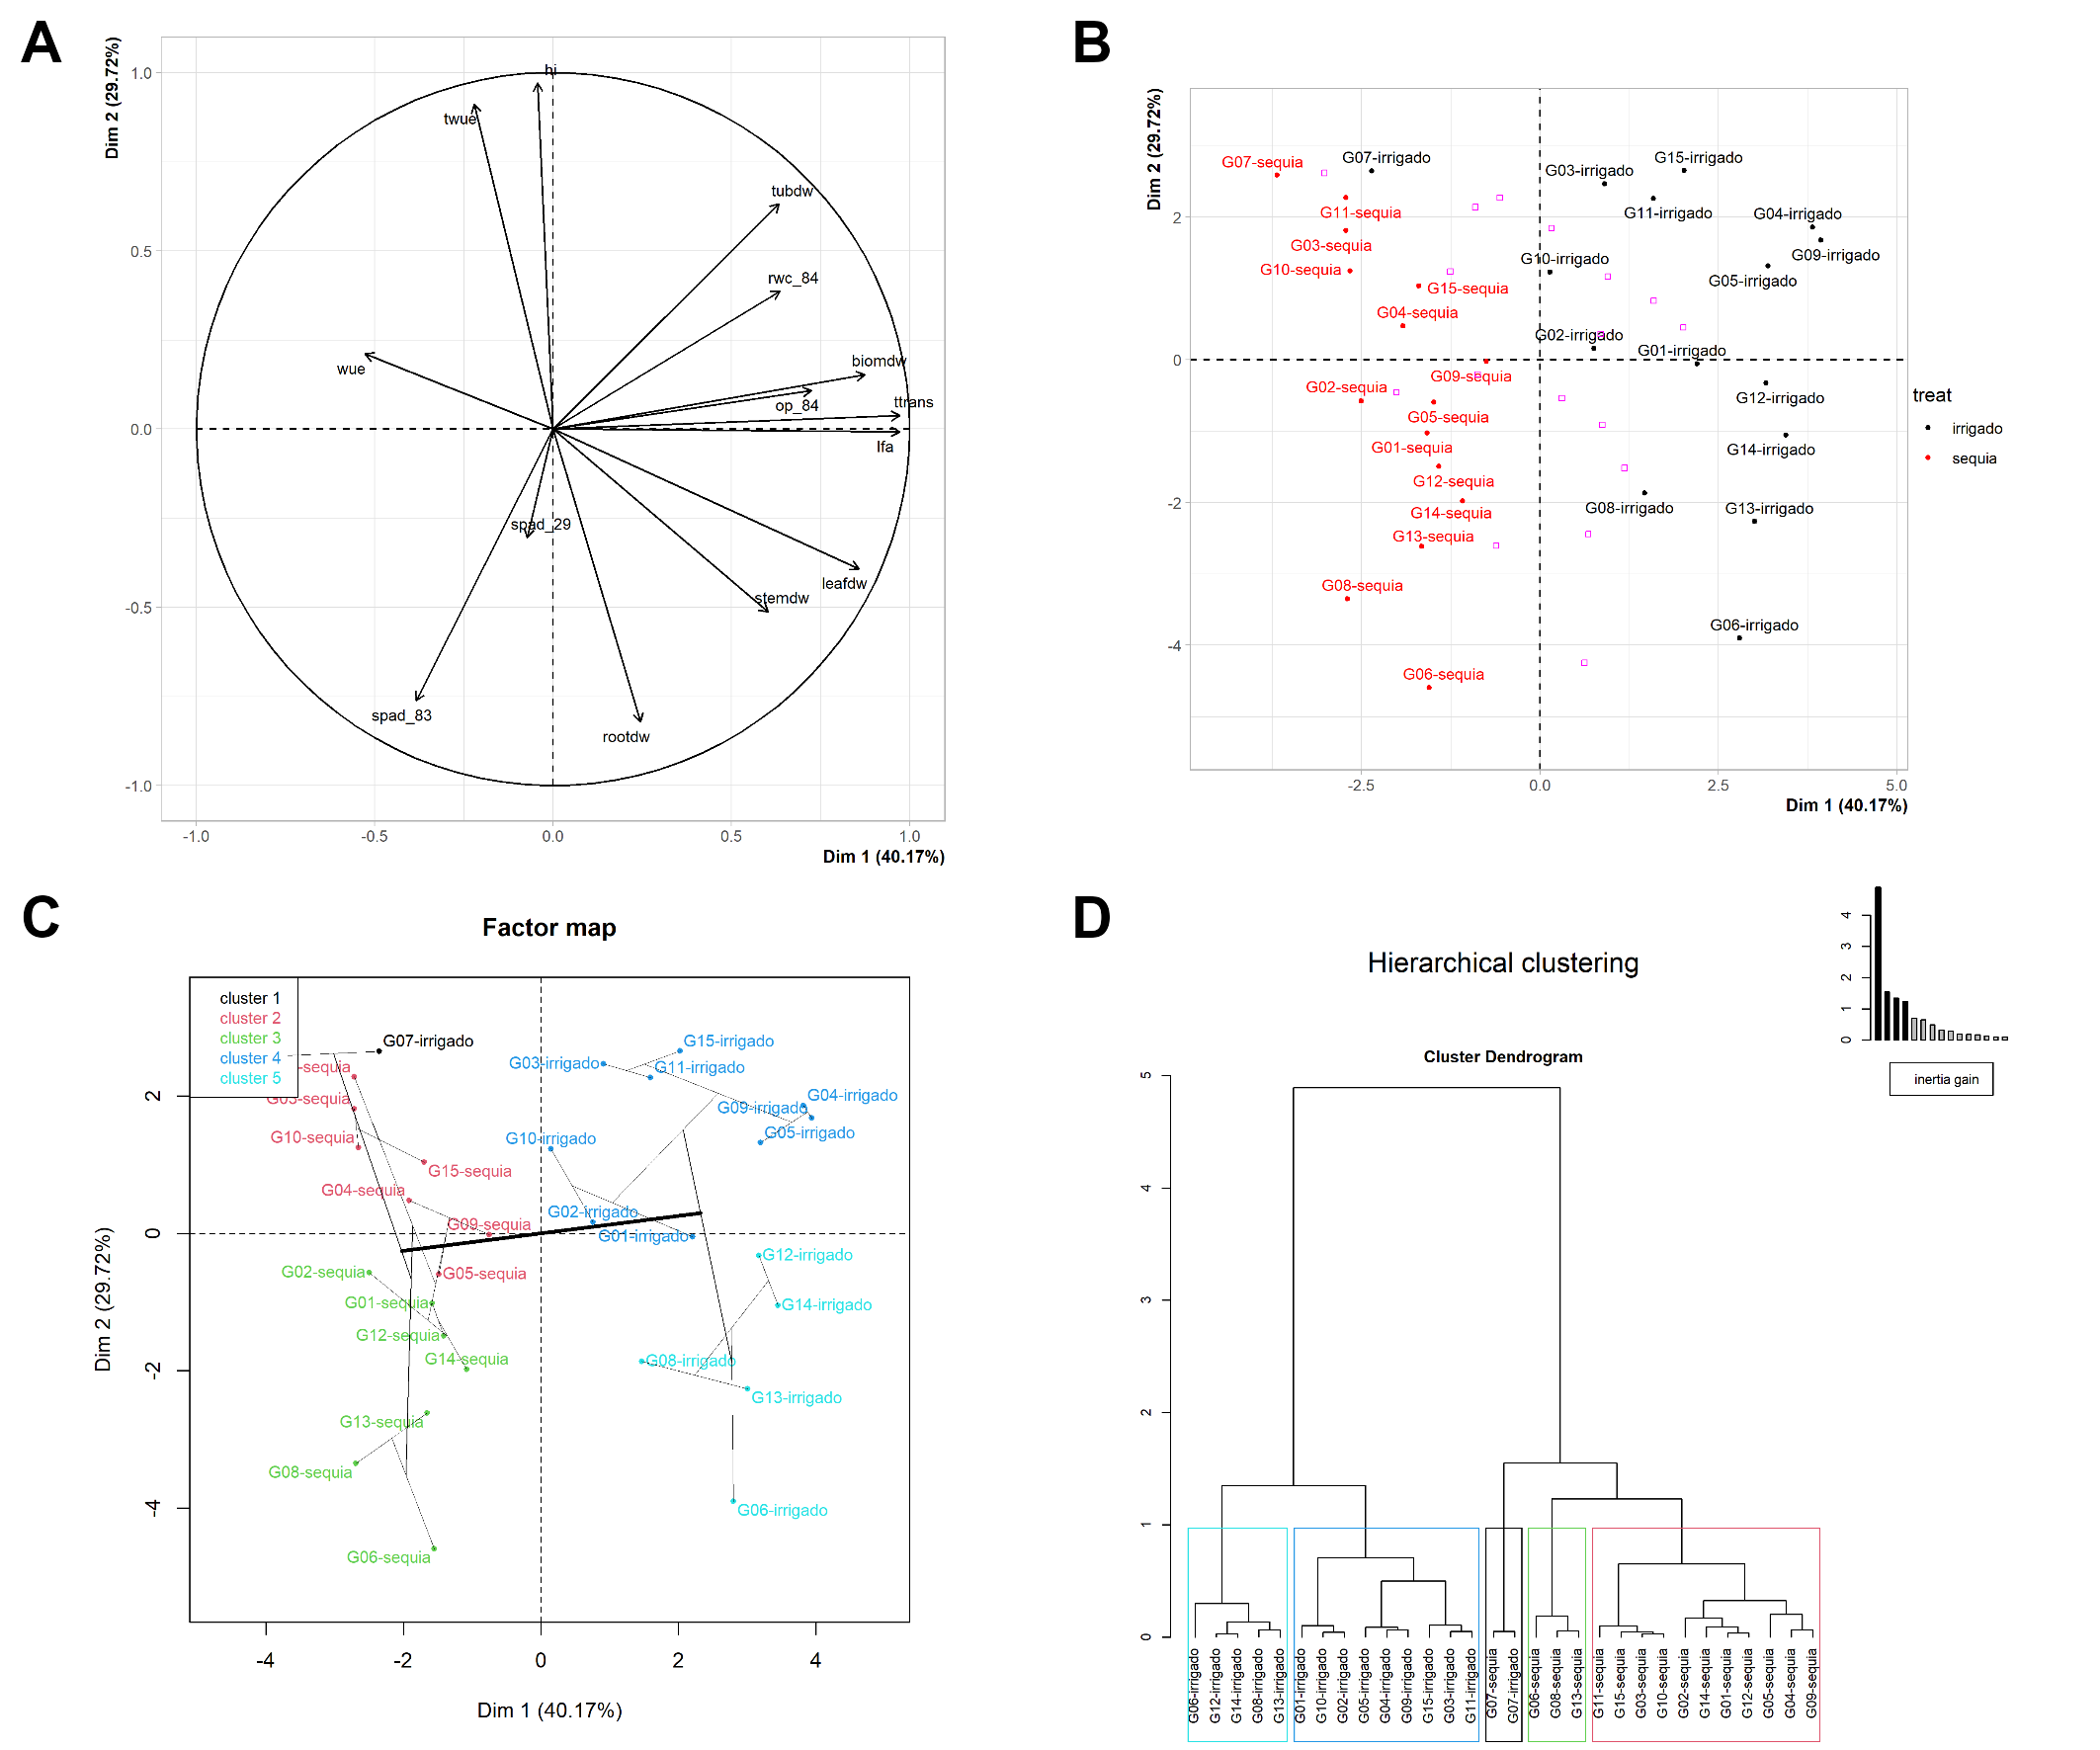
\includegraphics[width=0.98\linewidth]{files/fig-03} 

}

\caption{Multivariate Analysis: Principal component analysis and hierarchical clustering analysis.}(\#fig:mv)
\end{figure}
  </main><aside class="col-md-3"><nav id="toc"><h2>On this page</h2>
    </nav></aside></div>



    <footer><div class="pkgdown-footer-left">
  <p>Desarrollado por <a href="https://lozanoisla.com/" class="external-link">Flavio Lozano-Isla</a>.</p>
</div>

<div class="pkgdown-footer-right">
  <p>Site built with <a href="https://pkgdown.r-lib.org/" class="external-link">pkgdown</a> 2.0.9.</p>
</div>

    </footer></div>

  

  

  </body></html>
